% Chapitre sur le rapport d ingenierie :


\chapter{Rapport d'ingénierie} 


\section*{Introduction}
Ce PFE conclut les cinq années d'étude à l'INSA de Lyon. 
Il s'agit de démontrer des capacités d'adaptation,
d'innovation et d'initiative propres à un ingénieur.

Les laboratoires ont besoin de l'expertise d'ingénieurs
pour résoudre des problème techniques, qui se posent du fait de l'utilisation de matériel hautement sophistiqué.
Notamment, au Megason Lab, ce sont principalement des ingénieurs qui développent le programme de visualisation de données. 
Les problèmes d'acquisitions d'images biologiques révèlent aussi des défis techniques.
 
\section*{Objectifs}

Les objectifs initiaux étaient centrés principalement sur la recherche.
Cependant, le Megason lab cherche au maximum à intégrer les avancées en traitement de l'image aux outils qu'il conçoit,
 notamment au programme Gofigure2. Cela entraine des contraintes vis à vis des outils de développements. 
 Il a donc fallu me former afin que je devienne un programmeur avancé en {\C++}. 
 
J'ai ainsi commencé mon PFE en tant que membre de l'équipe de développement de Gofigure2.
 Les objectifs étant d'apprendre les différentes librairies utilisées par le programme, pour mettre au point un système de plugins
 \footnote{En informatique, un plugin ou plug-in (aussi nommé module d'extension, greffon ou plugiciel au Québec) est un logiciel qui complète un logiciel hôte pour lui apporter de nouvelles fonctionnalités. Notamment, pour le logiciel Gofigure2, les plugins seront des algorithmes de traitement d'images.}. 
 Ma mission était de créer une librairie de comparaison d'images, afin d'inclure aux plugins, un aperçu à la Photoshop.

Dans le cadre de ma participation au développement de Gofigure2,
 j'ai aussi proposé un protocole de travail avec un nouveau programme de gestion de versions : Git.
 Il s'agissait tout d'abord d'apprendre à utiliser Git, pour ensuite transmettre ce savoir et enfin proposer une méthode de travail.

Mon PFE étant motivé par des objectifs de traitement de l'image, j'ai aussi travaillé sur l'amélioration
 des techniques d'acquisitions de données microscopiques.
 
 
\section*{Planning} 
 
Des objectifs, nous pouvons dégager des taches, que nous plaçons dans un diagramme de Gantt. Le diagramme présenté figure~\ref{fig:GanttPFEInge}, ne concerne que les tâches d'ingénierie, or le PFE était aussi un stage master avec des objectifs recherche. Le diagramme de Gantt général du PFE est donc présenté en annexe \ref{AnnexeGanttGlobal}.
 
\begin{figure}[h]
\begin{center}
\leavevmode
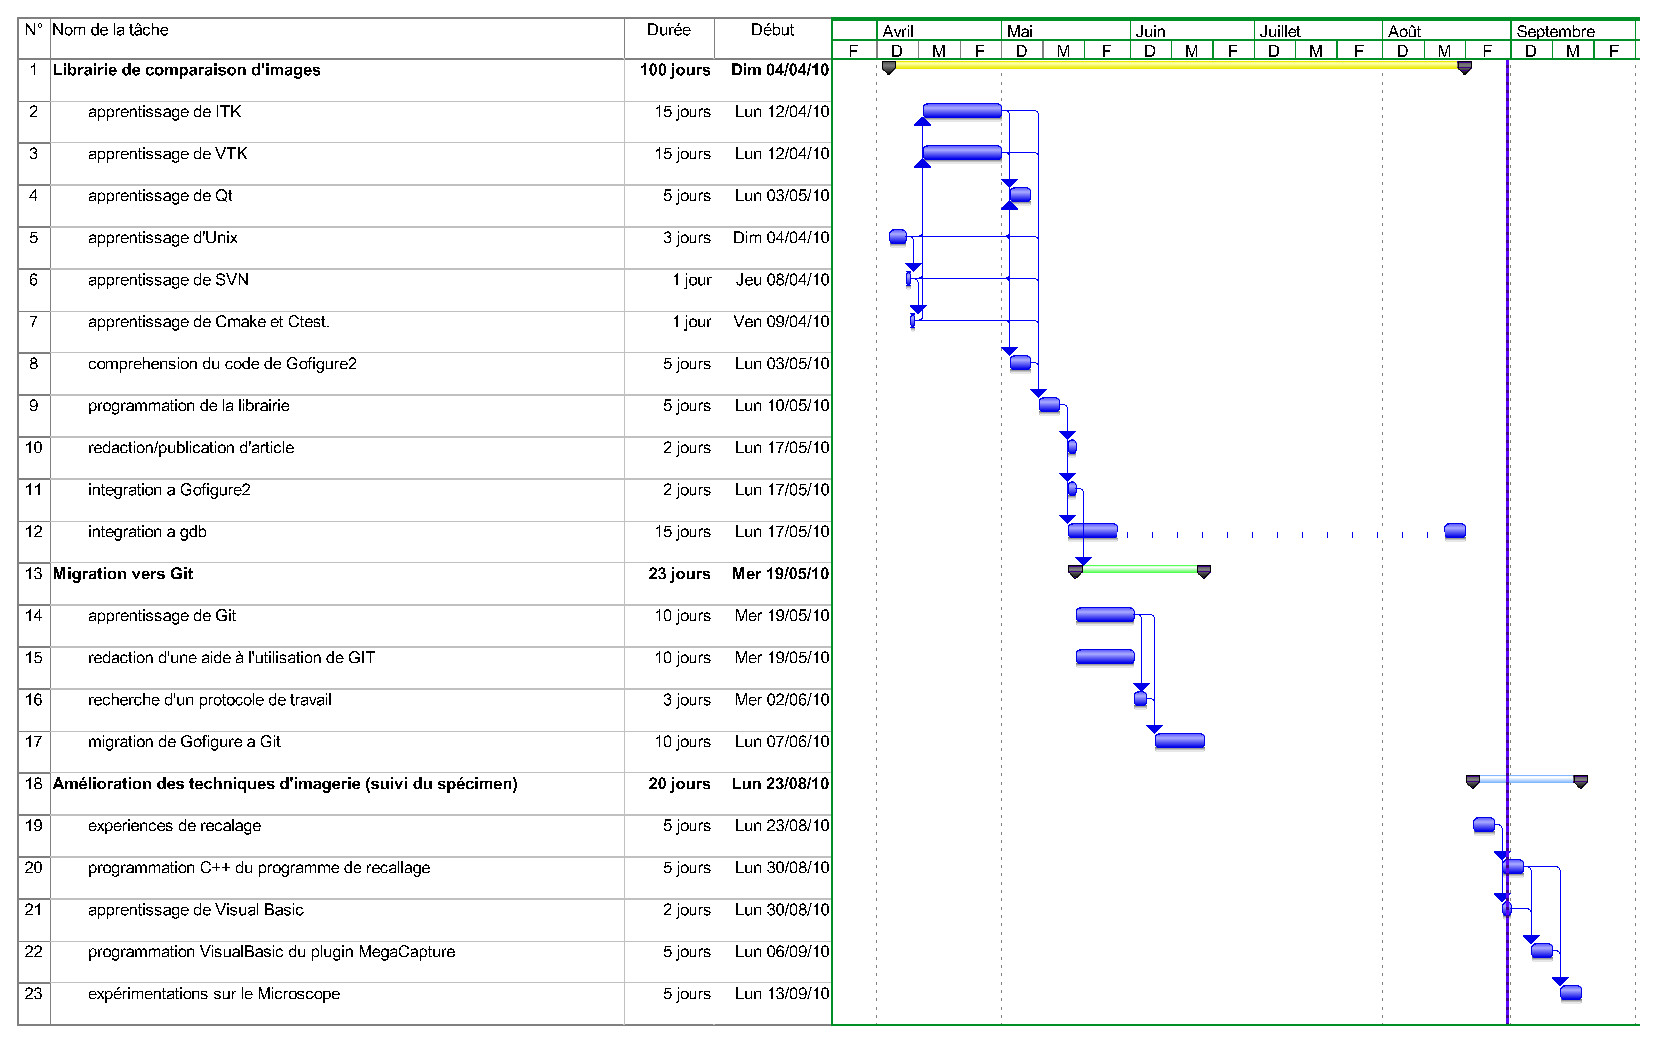
\includegraphics[angle=-90, width=0.95\textwidth]{pictures/GanttPFEInge}
\end{center}
\caption{Gantt de la partie ingénierie du PFE}
\label{fig:GanttPFEInge}
\end{figure}

%--------------------------------------------------
%             COMPARAISON
%--------------------------------------------------


\section{Création d'une librairie de comparaison d'images}

L'équipe d'informaticiens au Megason Lab est divisée en deux : deux ingénieurs travaillent sous la direction d'un docteur sur la
 création de l'outil de visualisation d'images microscopiques (GoFigure2), tandis qu'un autre docteur travaille sur
 des algorithmes de traitement d'image. Afin de travailler pour l'ensemble des informaticiens, le projet a deux objectifs
\begin{inparaenum}[(i)]
  \item faciliter le travail de développement d'algorithmes de traitement de l'image, et 
  \item s'intégrer au développement de GofiGure2.
\end{inparaenum}

La création de la librairie de comparaison d'images atteint ces deux buts (i) et (ii):\\ 
Il s'agit d'un programme utilisant le code source du projet Gofigure2, 
qui sera utilisé pour le développement des plugins de Gofigure2.
Cette librairie a enfin été spécifiquement développée pour compléter le projet de débugueur graphique de 
Matt MacCormick \cite{McCornic-VisualDebug}, afin de rendre cette librairie particulièrement utile
aux traiteurs d'image développant sous ITK.
Ce programme permet aussi de visualiser les traitements appliqués aux données
lors de l'exécution d'un algorithme de traitement d'images sous un environnement de debugging (gdb
\footnote{Un débogueur, débugueur ou encore debugger (de l'anglais), est un logiciel qui aide un développeur à analyser les bugs d'un programme. Pour cela, il permet d'exécuter le programme pas-à-pas, d'afficher la valeur des variables à tout moment, de mettre en place des points d'arrêt sur des conditions ou sur des lignes du programme ...\\
Le GNU Debugger également appelé gdb est le débogueur standard du \href{http://fr.wikipedia.org/wiki/Projet_GNU}{projet GNU}.} ).


\subsection{Cahier des charges}

Nous spécifions l'ensemble des tâches réalisées au cours du PFE avec la méthode APTE. Celle ci nous permet de définir les fonctions à remplir pour parvenir à un objectif. L'objectif est spécifié par le diagramme Bête à cornes (figure~\ref{fig:BACCompare}), tandis que les fonctions sont décrites dans l'analyse du diagramme pieuvre(figure~\ref{fig:PIEUVRECompare}).

\begin{figure}[h]
\begin{center}
\leavevmode
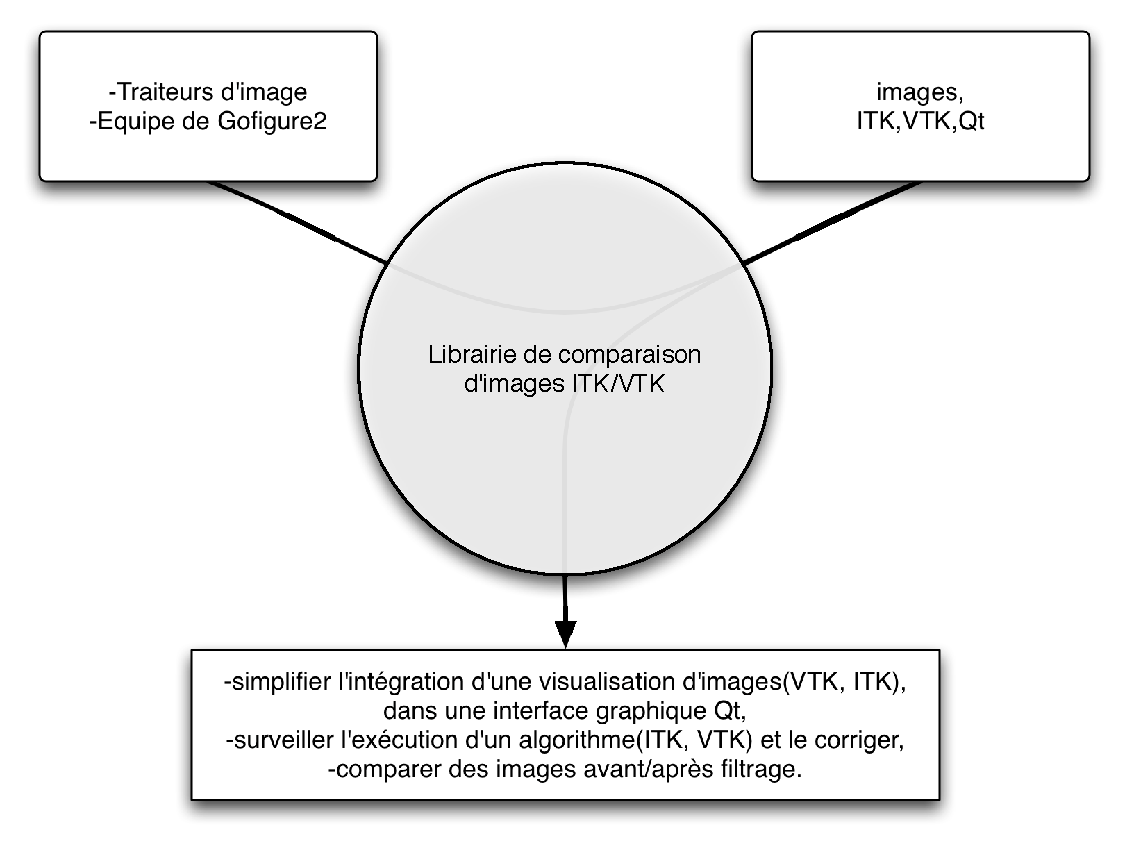
\includegraphics[width=0.95\textwidth]{pictures/CompareBAC}
\end{center}
\caption{Bête à cornes (méthode {APTE\textregistered}) de la librairie de comparaison d'images}
\label{fig:BACCompare}
\end{figure}

L'analyse de la Bête à cornes consiste en répondre aux questions :
\begin{inparaenum}[(i)] 
  \item pourquoi cherche-t'on à atteindre ce but ?
  \item et qu'est ce qui pourrait faire disparaitre ou évoluer le projet ?
\end{inparaenum}

Le programme Gofigure2 va bientôt disposer d'une interface pour créer des plugins afin de traiter des images microscopiques.
Le développement d'une librairie de visualisation et de comparaison est donc nécessaire
pour contrôler les paramètres des algorithmes inclut dans les plugins.

De plus, lors du développement d'algorithmes,
il est souvent nécessaire, lors de la phase de test et d'évaluation,
de visualiser l'état des données traitées, pendant l'exécution du programme.
Les algorithmes sont la plupart du temps prototypés en \C++ au Megason Lab, et la visualisation de données n'est pas triviale.
Il faut souvent ajouter une dizaine de lignes de codes pour pouvoir sauvegarder une image.
Une telle tâche est fastidieuse, et ce projet permettrait de visualiser
des données lors de l'exécution du programme, sans rajouter de code ni le recompiler !\\

De par mon implication dans l'équipe de Gofigure2 et
comme je vais être amené à développer des algorithmes en {\C++},
coder une librairie de comparaison d'images me permettra de me former aux outils utilisés au Megason Lab,
tout en créant un outil indispensable pour mes travaux futurs.

\begin{figure}[h]
  \begin{center}
  \leavevmode
  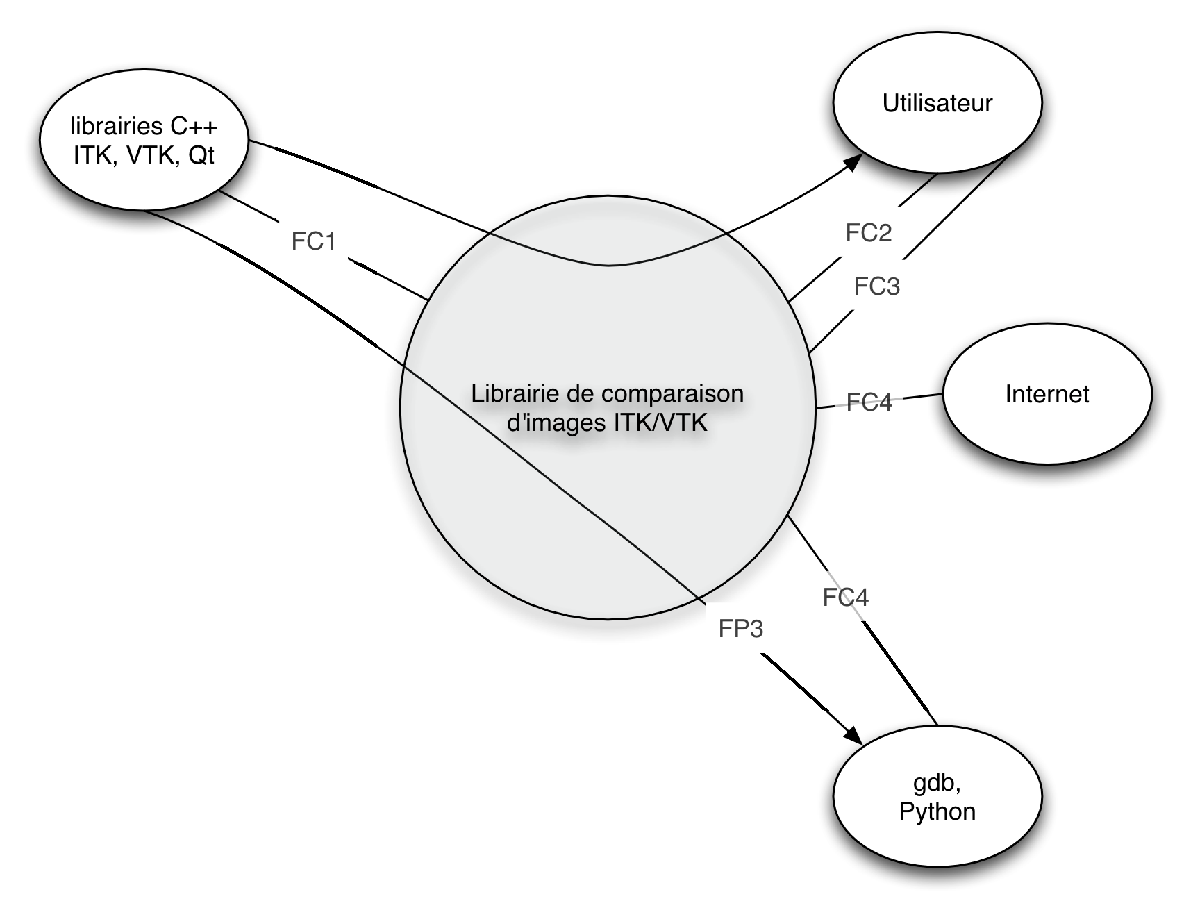
\includegraphics[width=0.95\textwidth]{pictures/ComparePIEUVRE}
  \end{center}
  \caption[Diagramme Pieuvre (méthode {APTE\textregistered}) de
    la librairie de comparaison d'images]{Diagramme
    Pieuvre (méthode {APTE\textregistered})
    de la librairie de comparaison d'images
  \small
  \textbf{Fonctions principales :}\\
  FP1 : visualiser des données (fichiers ou en mémoire) provenant 
    de VTK et ITK dans Qt\\
  FP2 : synchroniser la visualisation de plusieurs images\\
  FP3 : débuguer visuellement des pipelines ITK et VTK dans gdb\\
    \textbf{Fonctions contraintes :} \\
  FC1 : être compatible avec VTK, ITK et Qt\\
  FC2 : proposer une interface simple, une documentation, des exemples, et être
    facilement modifiable\\
  FC3 : être visible sur internet\\
  FC4 : être compatible avec Python pour interfacer avec gdb}
  \label{fig:PIEUVRECompare}
\end{figure}


\clearpage


Une analyse du diagramme pieuvre est ensuite donnée. Nous répondons aux questions de la méthode {APTE\textregistered}, pour chaque fonction :
\begin{inparaenum}[(i)] 
  \item dans quel but existe-t-elle ?
  \item à cause de quoi existe-t-elle ?
  \item pourrait-elle évoluer ou disparaitre ?
\end{inparaenum}


\paragraph*{FP1} :\\ visualiser des données (fichiers ou en mémoire) provenant de VTK et ITK dans Qt
\begin{itemize}
  \item Existe pour afficher les résultats des traitements réalisés par des plugins ITK/VTK dans Gofigure2.
  \item Existe à cause de la nécessité pour l'utilisateur d'avoir une visualisation dans une interface construite.
  Existe du fait de la complexité actuelle de l'utilisation d'ITK et VTK avec Qt. 
  \item Pourrait disparaitre si une librairie plus efficace et simple de visualisation était crée.
\end{itemize}

\paragraph*{FP2} :\\ synchroniser la visualisation de plusieurs images
\begin{itemize}
  \item Existe pour comparer pixel(voxel) par pixel plusieurs images.
  \item Existe à cause du besoin des traiteurs d'image d'une telle comparaison.
  \item Pourrait évoluer si VTK ou le moteur 3D utilisé vtkINRIA3D\cite{vtkINRIA}
  proposaient des solutions simple de synchronisation de visualisations.
\end{itemize}

\paragraph*{FP3} :\\ débuguer visuellement des pipelines ITK et VTK dans gdb
\begin{itemize}
  \item Existe pour permettre au programmeur de rapidement visualiser des images
   à différents points d'une pipeline ITK ou VTK.
  \item Existe à cause du besoin de débuguer les algorithmes de traitement d'image,
  et de visualiser les images d'une manière compréhensible par un humain.
  \item Pourrait évoluer si ITK, gdb ou Python évoluent.
\end{itemize}

\paragraph*{FC1} :\\ être compatible avec VTK, ITK et Qt
\begin{itemize}
  \item Existe pour permettre à l'application de fonctionner.
  \item Existe car ces 3 librairies sont complémentaires et souvent utilisées conjointement dans une même application.
  \item Pourrait disparaitre si une librairie regroupant les fonctions d'ITK, VTK et Qt était crée, et si Gofigure2 l'utilisait.
\end{itemize}

\paragraph*{FC2} :\\ Proposer une interface simple, une documentation, des exemples, et être facilement modifiable
\begin{itemize}
  \item Existe pour permettre à un utilisateur d'utiliser, comprendre et modifier la librairie.
  \item Existe à cause du fait qu'un code mélant ITK, VTK, et Qt n'est pas trivial.
  \item Pourrait évoluer avec la librairie.
\end{itemize}

\paragraph*{FC3} :\\ être visible sur internet
\begin{itemize}
  \item Existe pour permettre à un maximum de programmeur de télécharger la librairie et l'utiliser.
  \item Existe car la librairie est open-source et s'améliore avec les contributions d'autres utilisateurs.
  \item Pourrait disparaitre si la librairie venait à ne plus être publique.
\end{itemize}

\paragraph*{FC4} :\\ être compatible avec Python pour interfacer avec gdb
\begin{itemize}
  \item Existe pour permettre l'intégration à gdb et le débuguage visuel des pipelines ITK et VTK.
  \item Existe car le débugueur gdb nécessite une interface python 
  pour interpréter les données en provenance 
  des pipelines ITK et VTK dans un programme externe.
  \item Pourrait disparaitre si gdb n'utilisait plus Python 
  pour interfacer avec des programmes externes.
\end{itemize}

\subsection{Les outils utilisés}
Afin de pouvoir programmer ce projet,
il a été nécessaire d'apprendre à utiliser un certain nombre d'outils,
de librairies et concepts {\C++}. Cet apprentissage a été une
partie importante de mon PFE, me permettant d'acquérir de
nouvelles compétences en sciences informatiques.
\subsubsection{Les librairies \C++}
Il existe un grand nombre de fonctions déjà codées en {\C++}.
Dans une optique de standardisation et d'efficacité, il est important d'apprendre
à utiliser des librairies contenant les fonctions utiles au programme que l'on crée.

Le projet utilise trois grandes librairies :
\begin{description}
  \item[Insight ToolKit (ITK)] qui est spécialisée dans le traitement d'image. Nous utilisons cette librairie, 
  afin de supporter le type de données qu'elle stocke en mémoire.
  \item[Visualization ToolKit (VTK)] qui est spécialisée dans la visualisation d'images. 
  Nous utilisons cette librairie afin de supporter le type de données qu'elle stocke en mémoire,
  et aussi pour visualiser les données acquises par la librairie.
  \item[Qt]\cite{refQT} qui est spécialisée dans la création d'interfaces graphiques. 
  Nous avons rendu notre travail directement compatible avec cette librairie
  pour permettre aux utilisateurs de l'intégrer dans n'importe quelle application développée avec Qt.
  \item[vtkINRIA3D]{\cite{vtkINRIA}} qui est le moteur 3D utilisé par Gofigure2\cite{refGofigure2},
  le programme développé au MegasonLab.
  Cette librairie permet d'explorer un volume tri-dimensionnel en affichant trois coupes selon des plans perpendiculaires.
  Simultanément, un objet tridimensionnel composé par ces trois coupes est affiché.
  La version présente dans Gofigure2 à été grandement modifiée.
\end{description}
Une description détaillée de ces librairies est présentée en annexe \label{AnnexeDescriptionITKVTKQT}.


\subsubsection{Les outils de programmation}
A partir d'un certain niveau, en {\C++}, il est indispensable de maitriser certains outils complexes. Ceux-la, après un temps
 d'apprentissage, augmentent grandement la productivité.
Les outils utilisés quotidiennement, dans le processus de développement d'applications au Megason lab sont :

\begin{description}
  \item[l'Unix Shell] : pratiquement tous les développeurs travaillent sur Linux
  car ce système inclut un grand nombre d'utilitaires
  standards pour un développement en {\C++}.
  Les outils de gestion de versions comme Subversion (SVN) ou Git, les outils de connexion réseau (ssh),
  des compilateurs pour les principaux langages sont installés par défaut sur la
  plupart des distributions Linux.
  Afin de pouvoir bénéficier au maximum de ce système, il est important de maitriser
  l'invite de commande.
  \item[CMake] : ce programme permet de définir des règles de compilation pour différents compilateurs, afin qu'un projet puisse
   compiler sur différents systèmes d'exploitation (Nous programmons des applications fonctionnant sur Windows, Linux et MacOs).
  \item[CTest] : Lorsque l'on travaille sur un projet volumineux, il est facile de "casser" le code. L'ajout de certaines fonctionnalités 
  peut modifier le comportement d'autres parties du programme d'une manière imprévue. L'outil CTest est utilisé au Kegason Lab, 
  pour tester la fiabilité du code. Ce programme télécharge régulièrement le code source, le compile, et effectue une batterie de tests
  des fonctionnalités du programme.
  \item[SVN] : les développeurs de Gofigure2 travaillent sur les mêmes fichiers simultanément. 
  Dans ce cadre, il est important de garder une trace des modifications apportées par chacun. Il faut aussi combiner ces changements, 
  et sauvegarder le projet sur un serveur accessible à tous. SVN est un programme de gestion de versions qui remplit toutes ces 
  fonctions.
\end{description}


\subsection{Résultats et travail futur}

La librairie créée est fonctionnelle. Elle remplit les fonctions présentées en introduction. Un exemple de code est donné, illustrant l'extrême simplicité d'utilisation de la librairie :\\
Ce code permet d'ouvrir deux images : l'une provenant de la librairie ITK, et l'autre de VTK, et de synchroniser leur visualisation.
\large
  \begin{lstlisting}[title={Utilisation simple de la librairie de comparaison d'images}]{CompareCodeSimple}
#include "itkImageFileReader.h"
#include "vtkMetaImageReader.h"
#include "QGoSynchronizedViewManager.h"
#include <QApplication>

int main(int argc, char** argv)
{
  QApplication app(argc, argv);

  // ITK
  typedef double InputPixelType;
  typedef itk::Image<InputPixelType, 3> InputImage3DType;
  typedef InputImage3DType::Pointer InputImage3DPointer;
  typedef itk::ImageFileReader<InputImage3DType> itkReaderType;
  itkReaderType::Pointer itkReader = itkReaderType::New();
  itkReader->SetFileName("image3DA.mha");
  itkReader->Update();
  // ==========================

  // VTK
  vtkSmartPointer<vtkMetaImageReader> reader3D = 
    vtkSmartPointer<vtkMetaImageReader>::New();
  reader3D->SetFileName(image3DB.mha);
  reader3D->Update();
  // ==========================

  //Librairie creee
  QGoSynchronizedViewManager* syncViewManage =
    new QGoSynchronizedViewManager();

  syncViewManage->newSynchronizedView
    ("VisualisationA", filter13D->GetOutput());

  syncViewManage->newSynchronizedView<InputPixelType>
    ( "VisualisationB", itkReader->GetOutput() );
    
  syncViewManage->Update();
  syncViewManage->show();
  syncViewManage->synchronizeOpenSynchronizedViews();
  // ==========================


  //Qt
  app.processEvents();
  int output = app.exec();
  // ==========================
  
  delete syncViewManage;
  return output;
}
  \end{lstlisting}
\normalsize

La librairie permet de charger une image en une ligne de code,
et prend trois lignes pour afficher les images chargées d'une manière synchronisée.
Cela passe simplement par la création d'un QObjet : le QGoSynchronizedViewManager !\\

Une interface graphique basique a été créée pour illustrer les fonctionnalités de la librairie. La figure~\ref{fig:CompareQuad} est une capture d'écran de cet example.\\
\begin{figure}[h]
\center
\includegraphics[width=1\textwidth]{pictures/CompareQuad}
\caption{Example "compareguiexample" sur MacOsX 10.6. Ce programe utilise la librairie graphique créée pendant le PFE. Ici, l'utilisateur compare deux jeux de données 3D.}
\label{fig:CompareQuad}
\end{figure}

En plus d'un article dans l'Insight Journal, d'un code abondamment commenté, et d'une panoplie d'exemples,
la librairie est délivrée avec une documentation en ligne.\\

Afin de prouver la robustesse des classes utilisées, une série de tests automatiques a été créée.
La librairie a été intégrée au code de Gofigure2, au seins de se librairie graphique (QGoGUI), et est également intégrée au débugueur graphique, en collaboration avec Matt MacCormick.\\

La librairie de comparaison d'images est une très bonne base à laquelle on peut ajouter de nombreuses fonctionnalités :
\begin{itemize}
  \item supporter des images vectorielles d'ITK,
  \item intégrer des filtres simples (gradient, inverse, seuillage...),
  \item ajouter un moteur de rendu 3D (par tracé de rayons par exemple...).
\end{itemize}






%--------------------------------------------------
%             Git
%--------------------------------------------------


\section{Migration de Gofigure de SVN à Git}

Le projet Gofigure, suivant la plupart des grands projets open-sources, va bientôt utiliser Git comme programme de gestion de sources.
Plus qu'un simple transfert, il s'agit d'un changement des méthodes de travail.
Il a donc fallu définir un protocole de travail sur Git 
afin d'effectuer certaines tâches d'une manière organisée et répétable. 

Je suis donc passé par une phase de découverte et d'apprentissage pour écrire un tutoriel 
afin d'expliquer le fonctionnement de Git a l'équipe informatique. J'ai ensuite travaillé sur la sélection et l'élaboration d'un "workflow"
pour l'équipe de programmateurs de Gofigure2.
J'ai enfin automatisé le transfert du code de SVN à Git en utilisant un serveur du Megason Lab.



\subsection{La gestion de versions}

Cette partie présente brièvement la gestion de versions et les philosophies existantes.

\paragraph{Le contrôle de versions} ou gestion de versions consiste en
la création d'un historique des modifications apportées à un projet.
Il est nécessaire de disposer d'un programme à cet effet,
surtout lorsque plusieurs personnes travaillent sur le même projet.
Il est ainsi possible de garder trace de toutes les modifications apportées.
Certains programmes de gestion de versions permettent
de modifier l'historique en annulant l'effet d'une modification erronée par exemple.

Les programmes récents de gestion de versions sont aussi utilisés
pour permettre à plusieurs développeurs de travailler 
sur le même fichier, ou sur des fonctionnalités différentes.

Il existe un vocabulaire particulier au gestion de versions.
Pour ce rapport, il est important de comprendre l'analogie de l'arbre couramment utilisée.
Le tronc (trunc) contient généralement la dernière version commune du projet.
De ce tronc, les programmeurs créent des branches pour apporter des changements.
Ces branches sont des copies du tronc.
L'action de sauvegarder dans l'historique les changements apportés au projet se nomme "committer" (to commit).
L'action de fusionner une branche au tronc
(et ainsi rapporter tous les changements effectués sur une branche au tronc), s'appelle le merge.
Dans les  "anciens" programmes de gestion de versions,
les changements (commits) sont souvent directement faits sur le tronc.
Cela crée des problèmes de conflits
(plusieurs utilisateurs auraient changé d'une manière différente le même fichier, par exemple).

Le code source est souvent stocké sur un serveur en ligne.
Ainsi, le programme de gestion de versions est aussi utilisé
pour publier le code sur internet, par l'intermédiaire de sites spécialisés
(Sourceforge, Github, Gitorious, GoogleCode...).


\subsubsection{Les deux philosophies de gestion de versions} 

Il existe pour l'instant deux types de systèmes de gestion de versions : 
les systèmes basés sur une architecture centralisée,
et les systèmes basés sur une architecture décentralisée.

La gestion centralisée est basée sur un serveur qui contient la copie de référence des fichiers, 
et tout l'historique du projet. 
Les programmeurs n'ont sur leur ordinateur, que la dernière version du projet. 
Ce mode de fonctionnement nécessite une connexion au serveur pour faire avancer le projet.

La gestion décentralisée, par opposition, n'impose théoriquement pas de serveur central.
Les programmeurs disposent chacun d'une copie complète du projet sur leur ordinateur
qu'ils modifient à leur guise et synchronisent avec d'autres programmeurs.
Ce mode de fonctionnement permet de travailler sans connexion au serveur.

Il est possible de trouver une comparaison détaillée des deux philosophies sur
\href{http://informatique.in2p3.fr/?q=node/333}{le site de l'IN2P3}.


\subsubsection{Avantages de Git sur la concurrence}

Git n'est pas le seul programme de contrôle de version,
\href{http://en.wikipedia.org/wiki/Comparison_of_revision_control_software}{Wikipédia} en liste plus d'une trentaine !
Son principal concurrent est Mercurial, qui est aussi un programme de gestion de versions décentralisé,
plus simple mais disposant de moins de fonctionnalités, et Subversion, qui adopte la philosophie centralisée.

Cependant, en plus d'être l'un des programme de gestion de versions les plus utilisé,
 il possède de nombreux avantages dont les principaux sont:
\begin{description}
  \item[rapidité] : Git utilise un protocole de communication bien plus efficace que SVN (a peu près 5 fois plus rapide). 
  De plus, les commits peuvent être sauvegardés sans connexion au serveur central.
  \item[économie] : Git utilise un algorithme de compression très performant : le code prend ainsi très peu de place.
  \item[développement en commun] : chacun peut travailler sur une sous partie du programme. La création de "branches" est facile et
  rapide. La mise en commun des changements est bien mieux gérée que sur des programmes concurrents comme SVN.
  \item[développement décentralisé] : chacun possède une copie du code et peut travailler sans connexion internet. 
  Si le serveur subit une panne ou est indisponible, tout le monde peut continuer à travailler, et la recréation d'un serveur est triviale.
  \item[Souplesse] : Git permet de travailler sur un projet utilisant SVN (contrôle de version centralisée)
  en bénéficiant des avantages de la gestion de versions de projet décentralisée.
\end{description}

\subsection{Cahier des charges}

Maintenant que le principe de la gestion de versions a été présenté,
il nous est possible de définir un cahier des charges
pour le projet de migration vers Git de Gofigure2.
Nous utilisons une fois encore, la méthode {APTE\textregistered}.
Nous commencerons donc par définir le but principal du projet, pour passer à une analyse fonctionnelle.

\subsubsection*{Bête à corne de la migration vers Git}

\begin{figure}[h]
\begin{center}
\leavevmode
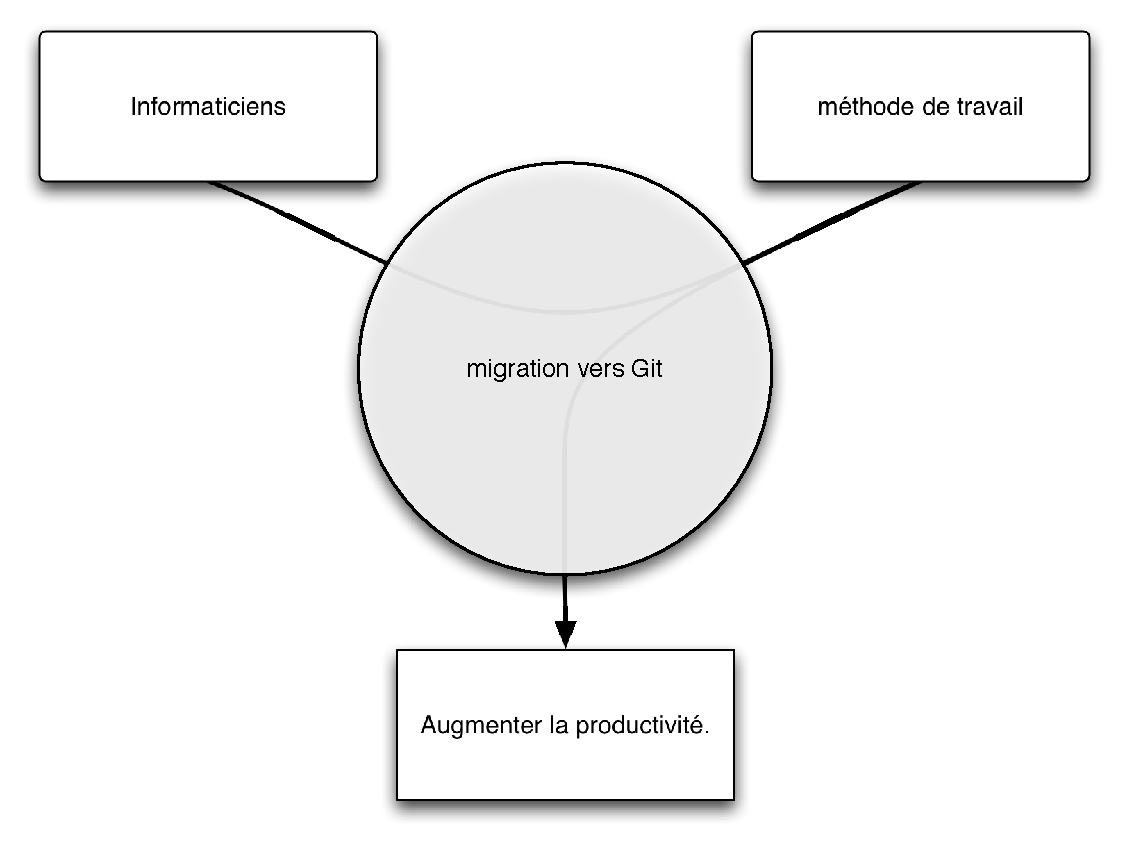
\includegraphics[width=0.95\textwidth]{pictures/GitBAC}
\end{center}
\caption{Bête à cornes (méthode {APTE\textregistered}) de la migration vers Git}
\label{fig:BACGit}
\end{figure}

Gofigure2 est un projet qui prend de l'ampleur,
nous souhaitons remplacer SVN par Git pour les multiples avantages
que ce dernier apporte à la gestion du projet et ainsi améliorer le protocole de travail.

La migration vers Git provient d'un besoin exprimé par la communauté de développeurs libres principalement.
Il permettra à l'équipe de Gofigure2 de travailler 
avec un nouveau standard de développement en suivant un workflow précis, qui facilite le travail en équipe.

Cette migration a été repoussée jusqu'à ce que Git soit adopté comme standard dans les communautés de développeurs.
Il est important de proposer un protocole de travail qui soit assez flexible pour permettre à l'équipe de le suivre,
tout au long de l'évolution de Gofigure2.
L'information donnée à l'équipe informatique devra évoluer en même temps que Git, et que le projet Gofigure2.


\subsubsection*{Diagramme pieuvre de la migration vers Git}

\begin{figure}[h]
\begin{center}
\leavevmode
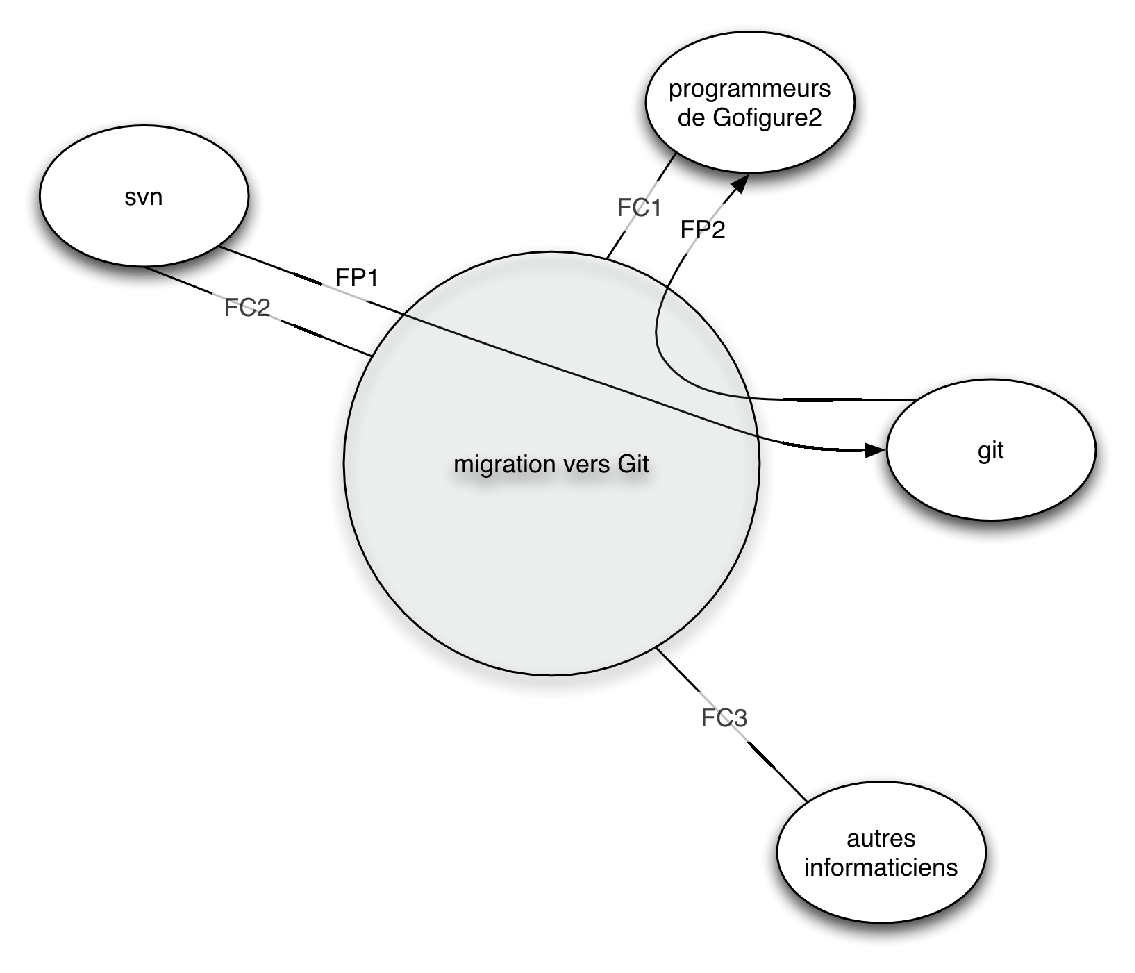
\includegraphics[width=0.95\textwidth]{pictures/GitPIEUVRE}
\end{center}
\caption[Diagramme Pieuvre (méthode {APTE\textregistered}) de la migration vers Git]{Diagramme Pieuvre (méthode {APTE\textregistered}) de la migration vers Git

\small
\textbf{Fonctions principales :}\\
FP1 : migrer le projet Gofigure2 de SVN à Git.\\
FP2 : proposer un workflow aux programmeurs de l'équipe de Gofigure2.\\
\textbf{Fonctions contraintes :} \\
FC1 : apporter une base de connaissance sur Git aux programmeurs de Gofigure2.\\
FC2 : rester compatible avec SVN.\\
FC3 : donner la possibilité à d'autres informaticiens de participer au projet.}
\label{fig:PIEUVREGit}
\end{figure}

\clearpage

Voici l'analyse du diagramme pieuvre du projet de migration de Gofigure2 vers Git :

\paragraph*{FP1} : migrer le projet Gofigure2 de SVN à git.
\begin{itemize}
  \item Existe pour améliorer le travail collaboratif sur Gofigure2.
  \item Existe à cause de l'apparition de nouveaux programmes performant combinant la gestion et la distribution de sources.
  \item Pourrait disparaitre si un nouveau modèle plus performant et intéressant pour l'équipe de Gofigure2 venait à apparaitre.
  Si la nouvelle version de SVN était adoptée par la communauté des développeurs libres.
\end{itemize}

\paragraph*{FP2} : proposer un workflow aux programmeurs de l'équipe de Gofigure2.
\begin{itemize}
  \item Existe pour structurer le travail avec Git.
  \item Existe du fait de l'extrême souplesse de Git : ce programme 
  permet de créer pratiquement n'importe quelle architecture de développement.
  \item Pourrait évoluer après une période d'étalonnage pour vérifier la pertinence du protocole.
  Si une norme venait à apparaitre.
\end{itemize}

\paragraph*{FC1} : apporter une base de connaissance sur Git aux programmeurs de Gofigure2.
\begin{itemize}
  \item Existe pour permettre aux programmeurs d'utiliser Git.
  \item Existe car Git est relativement complexe à prendre en main 
  pour un utilisateur habitué à d'autres programmes de gestion de source centralisés comme SVN.
  \item Pourrait disparaitre en partie si Git devenait trivial à l'usage.
  Il est important qu'une telle aide évolue avec Git, et avec le workflow de Gofigure2.
\end{itemize}

\paragraph*{FC2} : rester compatible avec SVN.
\begin{itemize}
  \item Existe pour permettre a un programmeur de continuer à utiliser SVN, et migrer vers Git progressivement.
  Existe aussi pour ouvrir les sources de Gofigure2 à plus de développeurs potentiels.
  \item Existe car tous les programmeurs n'utilisent pas (encore) Git.
  \item Pourrait disparaitre si SVN disparaissait.
\end{itemize}

\paragraph*{FC3} : donner la possibilité à d'autres informaticiens de participer au projet.
\begin{itemize}
  \item Existe pour permettre a un maximum de programmeur de télécharger Gofigure2, l'utiliser et participer à son développement.
  \item Existe car la librairie est open-source et s'améliore avec les contributions d'autres utilisateurs.
  \item Pourrait disparaitre si le protocole de travail n'était pas adapté à l'adjonction de code produit par un développeur tierce.
\end{itemize}


\subsection{Écriture du tutoriel}

Le tutoriel a été écrit sur le wiki de Gofigure2. Il s'agit de l'emplacement de prédilection pour les informations 
concernant la programmation et l'utilisation de Gofigure2. Le système du wiki, en plus de proposer une syntaxe simple 
pour créer des pages web formatées, permet aux lecteurs autorisés de modifier le contenu. 
Il existe aussi un système de feedback permettant aux lecteurs ayant mal compris le contenu, de contacter l'auteur.

Ce tutoriel remplit les fonction FC1 et FC3, présentées dans le diagramme Pieuvre(figure~\ref{fig:PIEUVREGit})

L'écriture d'un tel tutoriel se fait souvent dans un registre proche du langage familier,
le but étant de simuler des instruction données par un collègue ou un ami. 
Les instructions se doivent d'être relativement brèves, bien souvent le lecteur veut juste appliquer certaines fonctionnalités 
proposées par Git sans toujours vraiment chercher à comprendre ce qu'il fait. 
Il existe d'autres sources d'informations pour apprendre complètement le fonctionnement de l'application.
Le tutoriel ne se veut donc pas exhaustif, il propose juste une manière qui fonctionne d'utiliser Git,
à la manière d'un travail dirigé. Il a été écrit pendant ma phase d'apprentissage de Git. 
Il détaille les principales difficultés et écueils rencontrés. 

Le tutoriel est présent à cette adresse : \\
\url{http://sourceforge.net/apps/trac/gofigure2/wiki/Git}

\subsection{Proposition d'un protocole de travail}
Il a enfin fallu proposer un workflow (protocole de travail) 
qui définit la manière dont les programmeurs
doivent apporter des modifications au code source.
Afin de répondre aux fonctions FP2, FC2 et FC3 du diagramme pieuvre du cahier des charges, il fallait proposer un protocole qui :
\begin{enumerate}
  \item n'augmente pas trop la charge de travail,
  \item permette de bien suivre les modifications apportées par chacun. 
  \item permette au responsable du projet de corriger ou supprimer les changements apportés par les développeurs.
  \item corresponde à un standard.
\end{enumerate}

Le workflow proposé a été détaillé par \href{http://nvie.com/about }{Vincent Driessen} sur son \href{http://nvie.com/Git-model}{blog}.
Ce protocole découle assez naturellement de l'apprentissage de Git, il est donc simple.


Ce workflow, en plus d'être précisément détaillé, est techniquement viable. 
Voici le détail de l'organisation du projet Gofigure2 sous ce protocole.

Il existe deux branches principales : 
\begin{description}
  \item[\emph{master}] : cette branche stocke les versions stables du programme.
  \item[\emph{develop}] : cette branche contient la dernière version commune du programme, elle correspond au tronc.
\end{description}
Ces branches sont présentes sur le serveur central. Le développement du programme se fait sur la branche \emph{develop}, et lorsqu'une version stable est sur le point d'être produite, on sauvegarde l'état d'avancement du projet dans la branche \emph{master}.

Il existe ensuite une série de branches de support.
Ces branches ont une durée de vie limitée, et doivent fusionner avec d'autres branches pour finalement rejoindre \emph{develop} (le tronc), puis \emph{master}.
Elles ne sont pas forcément présentes sur le serveur central, cela dépend des équipes travaillant sur les différentes parties du programme.
\begin{description}
  \item[\emph{feature}] : cette branche contient le développement d'une fonction du programme. Elle est créée à partir de \emph{develop}, et une fois mature, refusionne avec \emph{develop}.
  \item[\emph{release}] : cette branche permet aux développeurs de travailler sur la correction de bugs, l'interface graphique, l'ajout de tests... les touches de dernière minute, avant la publication d'une nouvelle version du programme. Elle est créée lorsque la branche \emph{develop} contient toutes les fonctions attendues pour la nouvelle version du programme. Elle est créée à partir de la branche develop et une foi mature, fusionne avec la branche \emph{master}, et \emph{develop}.
  \item[\emph{hotfixes}] : cette branche particulière est créée à partir de la branche \emph{master}, lorsqu'une version publiée du programme contient un bug important qui ne peut attendre la prochaine version pour être corrigée. Elle refusionne avec la branche \emph{master} pour créer des "sous versions" (0.1.1 par exemple, est une sous version de 0.1.0). Cette branche particulière merge aussi avec la branche \emph{develop} pour appliquer la correction aux futures publications, et enfin, la branche \emph{release} si elle existe au moment de la réparation du bug.
\end{description}

Un cycle de développement simplifié devient donc, pour un programmeur :
\begin{figure}[h]
\begin{center}
\leavevmode
\includegraphics[width=0.95\textwidth]{pictures/Git_WorkflowSimple}
\end{center}
\caption{Diagramme simplifié du workflow proposé pour l'équipe de Gofigure2}
\label{fig:Workflow Git de Gofigure2}
\end{figure}

Il est important de noter que bien souvent, les informaticiens travaillent sur plusieurs choses à la fois,
et ce workflow permet ce genre d'organisation. 

\subsection{Mise en ouvre de la Migration vers Git}

Maintenant le worklflow définit, et l'aide mise en place, il faut mettre en œuvre la migration vers Git du projet. Nous devons choisir une plateforme pour héberger le projet, et mettre en place des liens entre le serveur SVN et le serveur Git.

\subsubsection{Github : une plateforme de travail collaboratif}

Github propose d'héberger gratuitement les projets open-sources. Les serveurs github sont administrables par un site
internet : \url{http://github.com/}. L'originalité de l'interface réside dans le réseau social proposé par le site. Il est possible de consulter les profils des programmeurs, de voir en temps réel l'avancement des projets sur lesquels ils travaillent. Le "fork" (copie d'un projet open source en vue de le modifier/l'améliorer) se fait en un click. Les collaborations se mettent en place d'un manière totalement transparente.

Nous avons donc opté pour cette plateforme, qui est une autre raison de la montée de Git comme programme de gestion de sources. Les connections sur ce site sont sécurisées par un protocole crypté (ssh)... Il est donc nécessaire d'effectuer certaines opérations de configuration avant de pouvoir utiliser les serveurs Git de Github. Les détails de la création d'un compte ont été repris dans le tutoriel à destination de l'équipe de Gofigure2.

\subsubsection{Automatisation de la migration vers Git}

Une fois l'organisation Gofigure2 créée sur Github, et les comptes des développeurs configurés, nous avons pu passer à la migration à proprement parler du projet.
Nous avons ensuite copié le contenu du serveur SVN de Gofigure2,
pour le traduire en un projet Git, en respectant le workflow proposé.

La figure~\ref{fig:MigrationGit} schématise la mise à jour du serveur Git avec les informations du serveur SVN.
Pour l'instant cette mise a jour est journalière.
Nous pourrions aussi envisager une mise à jour automatique à chaque modification du projet.
Un cycle de développement simplifie devient donc, pour un programmeur :
\begin{figure}[h]
\begin{center}
\leavevmode
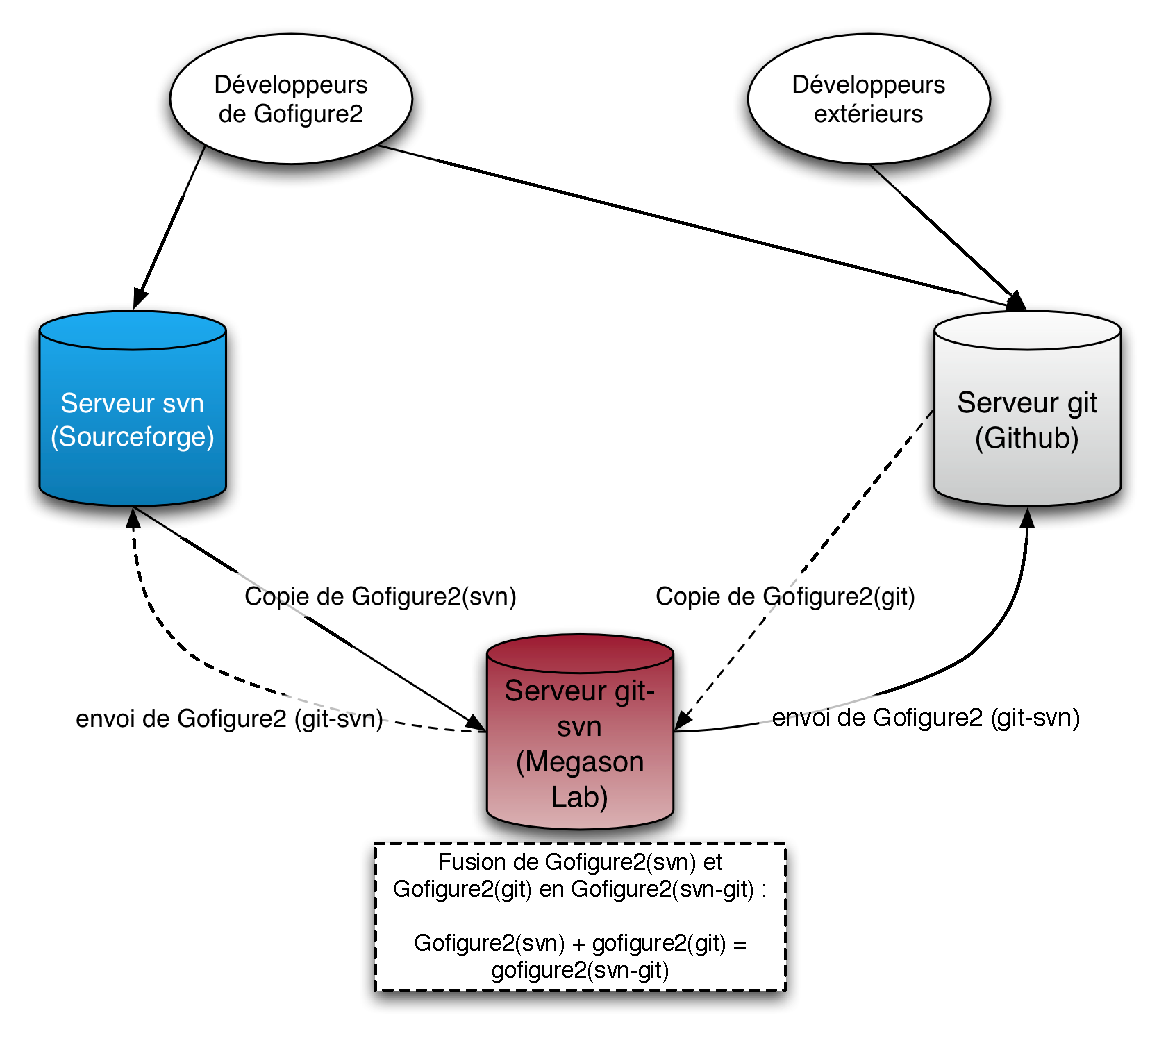
\includegraphics[width=0.95\textwidth]{pictures/GitTransfert}
\end{center}
\caption{Migration automatique de SVN vers Git via un serveur installé au Megason Lab}
\label{fig:MigrationGit}
\end{figure}
Le serveur du Megason Lab copie donc tous les jours les informations du serveur SVN.
Il transforme ces informations pour qu'elles soient compatibles avec le protocole de Git,
et conforme au protocole de travail proposé, puis les envoie sur le serveur de github.
Pour l'instant, les modifications provenant du serveur de Github (flèches pointillées)
sont manuellement intégrées au projet. Cependant, on peut facilement automatiser cette fusion des projets Git et SVN.

%for big figures in this chapter
\clearpage


%--------------------------------------------------
%             RECALAGE
%--------------------------------------------------

\section{Amélioration des techniques d'imagerie}

Ce projet part d'une initiative personnelle : ayant appris qu'il m'était possible de continuer à travailler au Megason Lab, sur des images acquises par le microscope confocal, je décidai d'améliorer la qualité des images acquises. En effet, ces données formeront la base de mes futures recherches, et trouver un moyen de les améliorer faciliterait d'autant mon travail.

J'ai donc adressé un problème très courant dans ce type d'imagerie : 
celui du mouvement incontrôlé du spécimen.
Cela a des conséquences catastrophiques sur la qualité des images : 
la région étudiée du spécimen peut être en dehors 
du champ microscopique\footnote{Un champ microscopique ou champ d'observation est la zone d'observation éclairée qui apparait au manipulateur lors d'une observation au microscope}
après quelques heures d'acquisition,
cela conduit aussi à des "sauts" violents causés par la remise en place manuelle de l'objectif.

Je vais tout d'abord prouver la validité d'un tel projet (projet de recalage), pour ensuite détailler la réalisation technique qu'il a engendrée.
\subsection{Cahier des charges}
Nous commençons par présenter la Bête à Cornes,
pour clarifier le but principal du projet. Nous présentons ensuite le diagramme pieuvre qui permet de détailler les fonctions du projet.

\subsubsection{Contrôle de la validité du projet}
\begin{figure}[h]
\begin{center}
\leavevmode
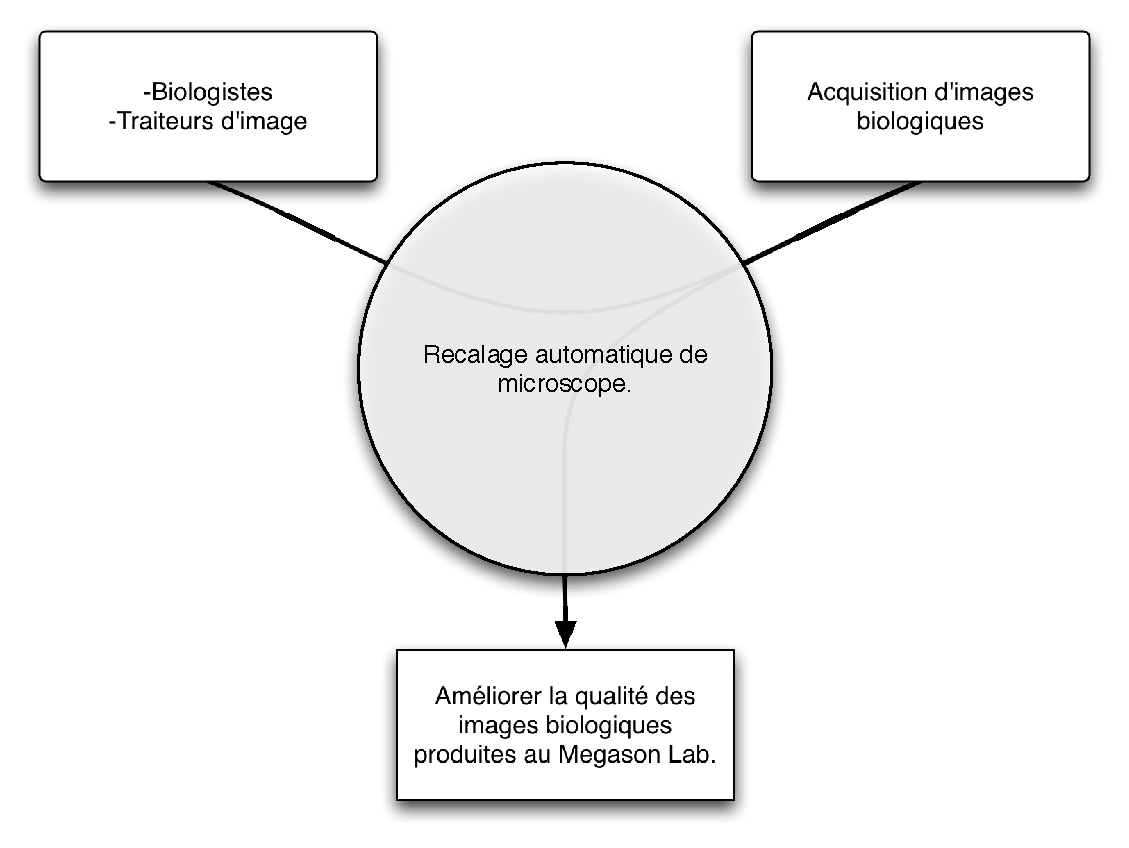
\includegraphics[width=0.95\textwidth]{pictures/RecalBAC}
\end{center}
\caption{Bête à cornes (méthode {APTE\textregistered}) du projet de suivi de spécimen}
\label{fig:BACRecal}
\end{figure}

La figure~\ref{fig:BACRecal} montre la Bête à cornes du projet de recalage d'images microscopiques.

La réalisation de ce produit résulte d'un besoin exprimé par les biologistes et traiteurs d'images.
Comme le spécimen change de forme durant la phase d'imagerie, il arrive qu'il ne soit plus dans le champ d'observation, ce qui est un réel problème pour les biologistes qui doivent contrôler l'alignement du microscope toutes les heures.
C'est aussi un problème pour les traiteurs d'images
car il arrive qu'un biologiste déplace en un mouvement un spécimen.
Cela invalide beaucoup de méthodes de suivi des objets imagés.

Ce projet, en automatisant l'alignement du microscope permet donc aux biologistes de moins surveiller l'acquisition,
et aux traiteurs d'images, de disposer de données exploitables.

Ce projet peut évoluer en accord avec les besoins des biologistes, et suivant l'évolution des techniques de recalage d'images.

\subsubsection{Expression fonctionnelle}

\begin{figure}[h]
\begin{center}
%\leavevmode
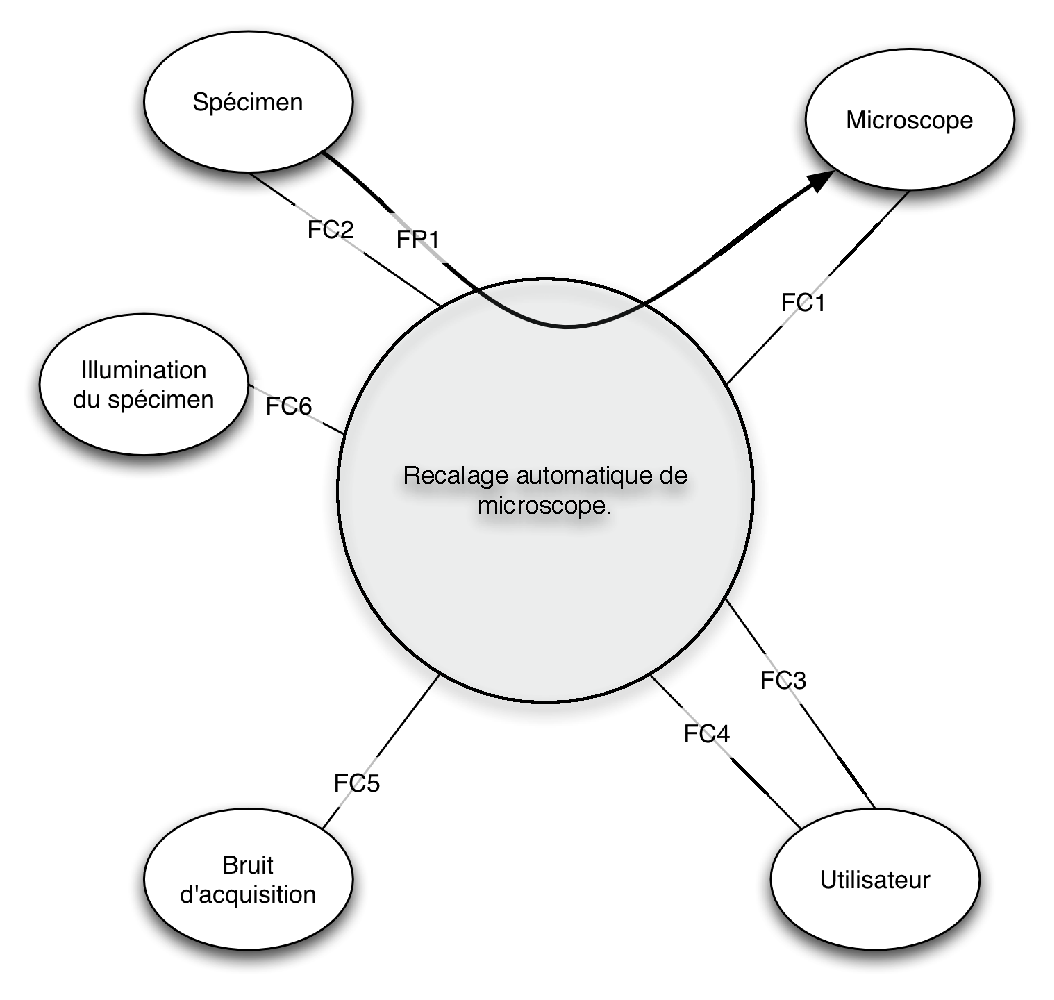
\includegraphics[width=0.9\textwidth]{pictures/RecalPIEUVRE}
\end{center}
\caption[Diagramme Pieuvre (méthode {APTE\textregistered}) du projet de suivi de spécimen]{Diagramme Pieuvre (méthode {APTE\textregistered}) du projet de suivi de spécimen

\small
\textbf{Fonction principale :}\\
FP1 : déplacer le microscope pendant l'acquisition en suivant le spécimen\\
\textbf{Fonctions contraintes :} \\
FC1 : compatible avec les logiciels utilisés\\
FC2 : robuste aux changements de forme du spécimen\\
FC3 : contenir une interface homme machine\\
FC4 : maintenable par l'équipe du Megason Lab\\
FC5 : robuste au bruit\\
FC6 : robuste aux changements d'illumination\\
FC7 : rapide}
\label{fig:PIEUVRERecal}
\end{figure}

\clearpage

La figure~\ref{fig:PIEUVRERecal} est le diagramme pieuvre du projet, que nous analysons :

\paragraph*{FP1} : déplacer le microscope pendant l'acquisition en suivant le spécimen.
\begin{itemize}
  \item Existe pour créer des images exploitables d'une manière fiable.
  \item Existe à cause de la nature du spécimen analysé, qui est vivant et en développement. 
  Il change donc de forme, grossit et se déplace, il faut donc suivre l'organe d'intérêt pendant le
  développement du spécimen.
  \item Pourrait disparaitre si le Megason Lab arrêtait d'imager des spécimens vivants.
  Si les microscopes avaient un champ de visualisation assez grand pour englober
  tout le spécimen et d'éventuelles marges de déplacement.
\end{itemize}

\paragraph*{FC1} : compatible avec les logiciels utilisés.
\begin{itemize}
  \item Existe pour fonctionner avec le matériel présent au Megason Lab.
  \item Existe à cause de la nature des logiciels utilisés au Megason Lab.
  \item Pourrait disparaitre si le logiciel de contrôle du Megason Lab était compatible avec n'importe quel langage informatique,
  en particulier le {\C++}.
\end{itemize}

\paragraph*{FC2} : robuste aux changements de forme du spécimen
\begin{itemize}
  \item Existe pour fonctionner sur différents spécimens analysés,
  et sur une période de temps étendue (le spécimen change de forme au cours du temps).
  \item Existe à cause de la nature des spécimens analysés au Megason Lab.
  \item Pourrait disparaitre si les spécimens n'évoluaient pas au cours du temps;
  si il existait un programme spécifique à chaque partie du spécimen.
\end{itemize}

\paragraph*{FC3} : contenir une interface homme machine
\begin{itemize}
  \item Existe pour interagir avec l'utilisateur.
  \item Existe à cause du besoin du programme de paramètres provenant de l'utilisateur.
  \item Pourrait disparaitre si le programme pouvait déterminer automatiquement les meilleurs paramètres.
\end{itemize}

\paragraph*{FC4} : maintenable par l'équipe du Megason Lab
\begin{itemize}
  \item Existe pour permettre aux autres chercheurs du Megason Lab de modifier/utiliser le programme.
  \item Existe car le développeur de l'application ne sera pas toujours présent pour la maintenir.
  \item Pourrait disparaitre si le programme se maintenait tout seul.
\end{itemize}

\paragraph*{FC5} : robuste au bruit
\begin{itemize}
  \item Existe pour permettre à l'algorithme de fonctionner en la présence de bruit
  \item Existe car le microscope produit des images bruitées.
  \item Pourrait disparaitre si le microscope produisait des images sans aucun bruit.
\end{itemize}


\paragraph*{FC6} : robuste aux changement d'illumination
\begin{itemize}
  \item Existe pour permettre à l'algorithme de fonctionner au cours du temps. 
  \item Existe car la fluorescence des spécimens décroit au cours du temps (phénomène de "bleaching"),
  et change d'une image à l'autre car le système d'illumination basé sur une probabilité d'absorption de photons.
  (le même phosphore n'absorbe pas toujours autant de photons avant de ré-émettre).
  \item Pourrait disparaitre si le bleaching disparaissait 
  et si nous contrôlions mieux l'absorption de photons par les phosphores du spécimen.
\end{itemize}

\paragraph*{FC7} : rapide
\begin{itemize}
  \item Existe pour permettre au microscope de faire des acquisitions peu espacées dans le temps
  \item Existe car l'alignement du microscope doit être fait avant l'acquisition.
  \item Pourrait disparaitre ou évoluer si nous intégrions une prédiction
  des déplacements futurs en fonction des déplacements précédents.
\end{itemize}

\subsection{Solutions techniques}

Le principe du programme est d'estimer le déplacement de structures notables dans l'image.
Une fois ce déplacement estimé, il s'agit de déplacer le spécimen afin de garder ces structures dans le champ du microscope.

\subsubsection{Estimation du déplacement du spécimen}
Nous utilisons une technique connue sous le nom de recalage d'images
\footnote{Le recalage d'images est une technique utilisée en traitement d'image pour mettre en correspondance les informations
provenant de deux images différentes. Afin d'aligner les images, une transformation géométrique est recherchée.
Cette transformation est choisie de manière à minimiser un critère de différence entre les images.
Le choix de la transformation et du critère de différence sont donc primordiaux.}
 pour estimer le déplacement du spécimen entre deux acquisitions (deux images) effectuées par le microscope : si nous trouvons une translation qui permette de passer d'une acquisition à l'autre, nous pouvons estimer le déplacement du spécimen.
Comme le microscope ne peut que déplacer le spécimen en translation, nous choisissons un recalage rigide qui évalue les translations selon les trois dimensions de l'espace, entre deux images.

Les techniques de recalage sont basées sur des critères de différence à minimiser.
On choisit ces critères de manière à ce que leur valeur soit élevée quand deux images sont mal alignées,
et faibles quand elles sont alignées. Notre programme teste différentes translations jusqu'à trouver une translation
qui donne une faible valeur du critère d'énergie.
Bien sûr, il n'est pas possible de calculer le critère de différence pour toute les translations possibles car cela prendrait trop de temps.
On choisit donc une technique qui "dirige" les estimations de manière à diminuer l'énergie
(la descente de gradient est une technique classique).
Enfin, afin que notre algorithme soit robuste vis à vis du bruit, et des changements de forme peu significatifs,
nous moyennons les images, puis réduisons la résolution des images moyennées.
Le facteur de réduction dépend de la taille du spécimen, des structures à analyser,
et de la résolution initiale des images acquises par le microscope.
\\
Le choix de la métrique est basé sur plusieurs critères : la simplicité d'utilisation (peu de paramètres),
la robustesse au bruit et aux changements d'illumination, et la robustesse aux changements de forme. Il faut enfin que cet algorithme soit rapide : le déplacement est calculé entre chaque acquisition, et doit prendre moins d'une minute au total. Ce choix est donc dicté par les contraintes FC2 à FC7 du diagramme pieuvre (figure\ref{fig:PIEUVRERecal}) !

Afin de sélectionner une métrique, plusieurs essais ont étés effectués, tout d'abord avec des déplacements simulés,
puis avec de réelles séquences d'images microscopiques.

\begin{figure}[h]
\begin{center}
\leavevmode
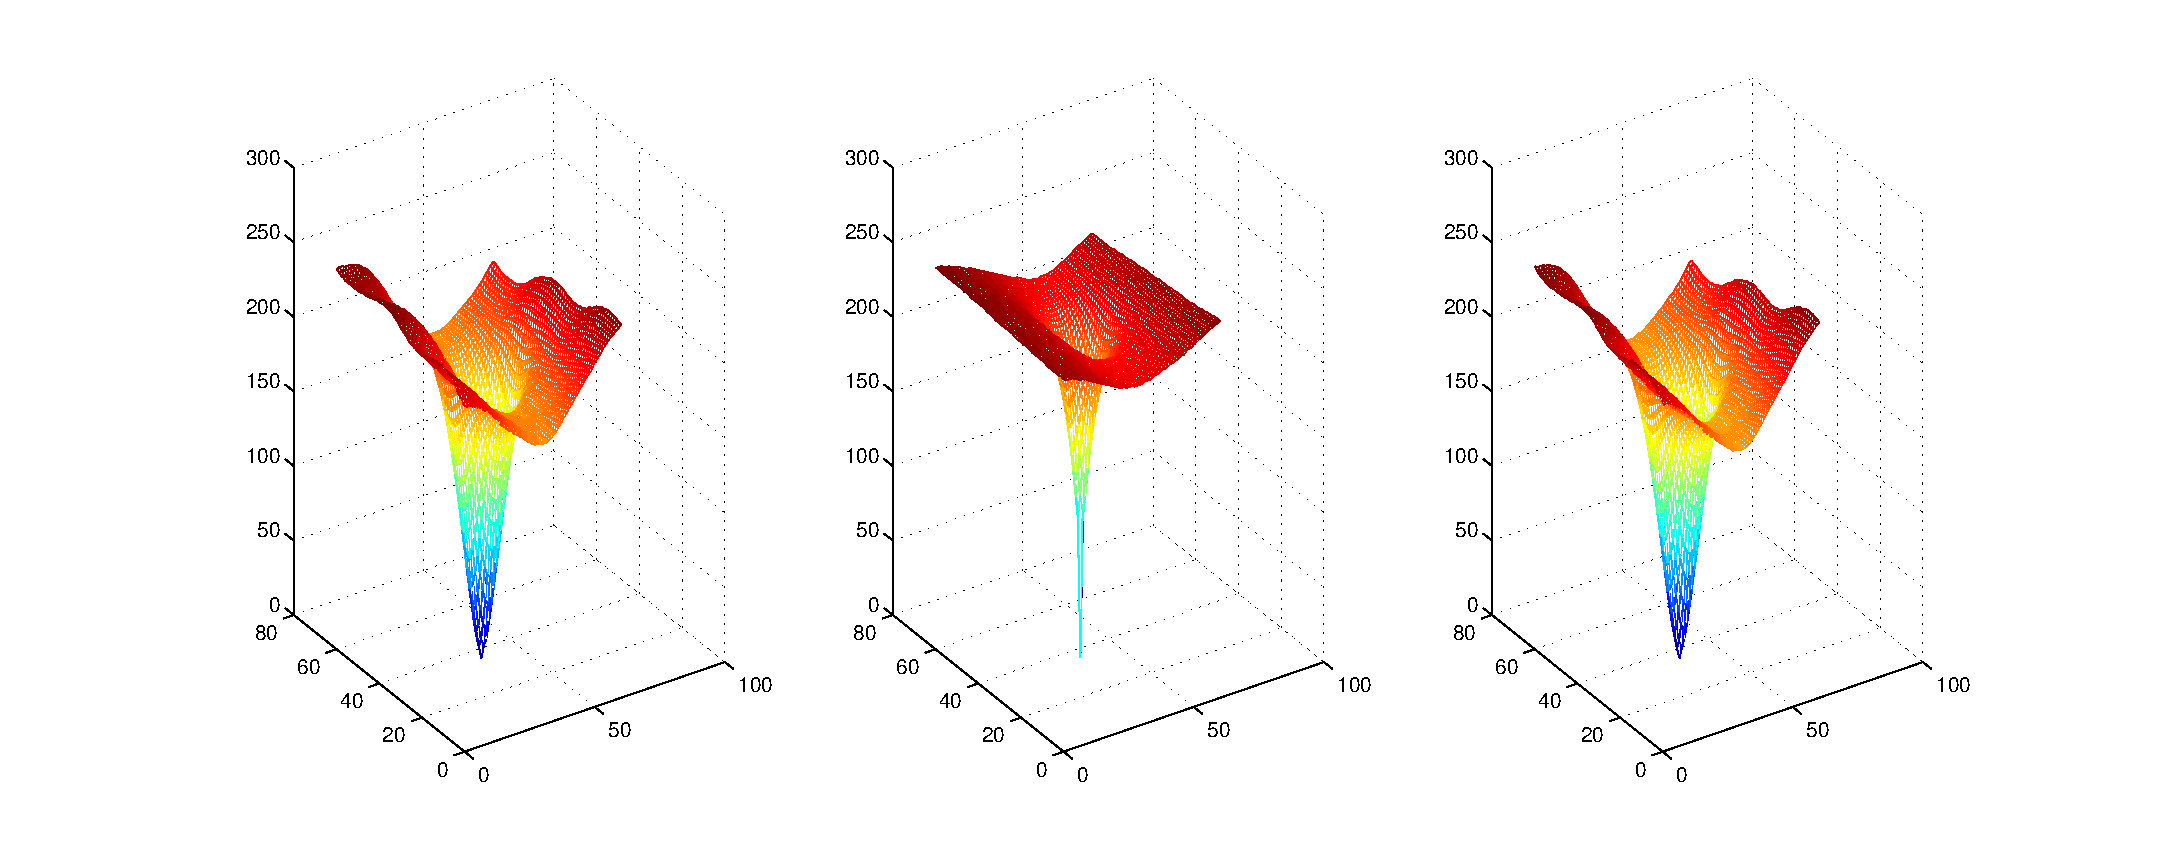
\includegraphics[width=0.95\textwidth]{pictures/Recal3DmetricsCMSArtificial}
\end{center}
\caption{Critères de différence pour une simulation de déplacement}{Valeur du critère de différence pour une simulation de déplacement du spécimen de 5 pixels en x et 5 pixels en y.\\
De gauche à droite :\\
critère de \href{http://www.itk.org/Doxygen/html/classitk_1_1NormalizedCorrelationImageToImageMetric.html}{corrélation normalisé};\\
critère d'information mutuelle de \href{http://www.itk.org/Doxygen/html/classitk_1_1MattesMutualInformationImageToImageMetric.html}{Mattes};\\
critère des \href{http://www.itk.org/Doxygen/html/classitk_1_1MeanSquaresImageToImageMetric.html}{moindres carrés}. }
\label{fig:RecalMetricSynthe}
\end{figure}


La figure~\ref{fig:RecalMetricSynthe} montre que le critère d'information mutuelle de Mattes semble être très précis : il présente un relief presque plat avec un pic correspondant à la translation synthétisée. Cependant, pour cette même raison, ce critère ne peut facilement recaler des images très différentes.
Le critère des moindres carrés, et le critère de corrélation normalisé donnent des résultats à peu près similaires. Il est important de noter que le critère des moindres carrés prend plus de temps à calculer, car il est évalué sur toute l'image (contrairement au critère d'information mutuelle de Mattes qui n'est évalué qu'en certains points aléatoires).


\begin{figure}[h]
\begin{center}
\leavevmode
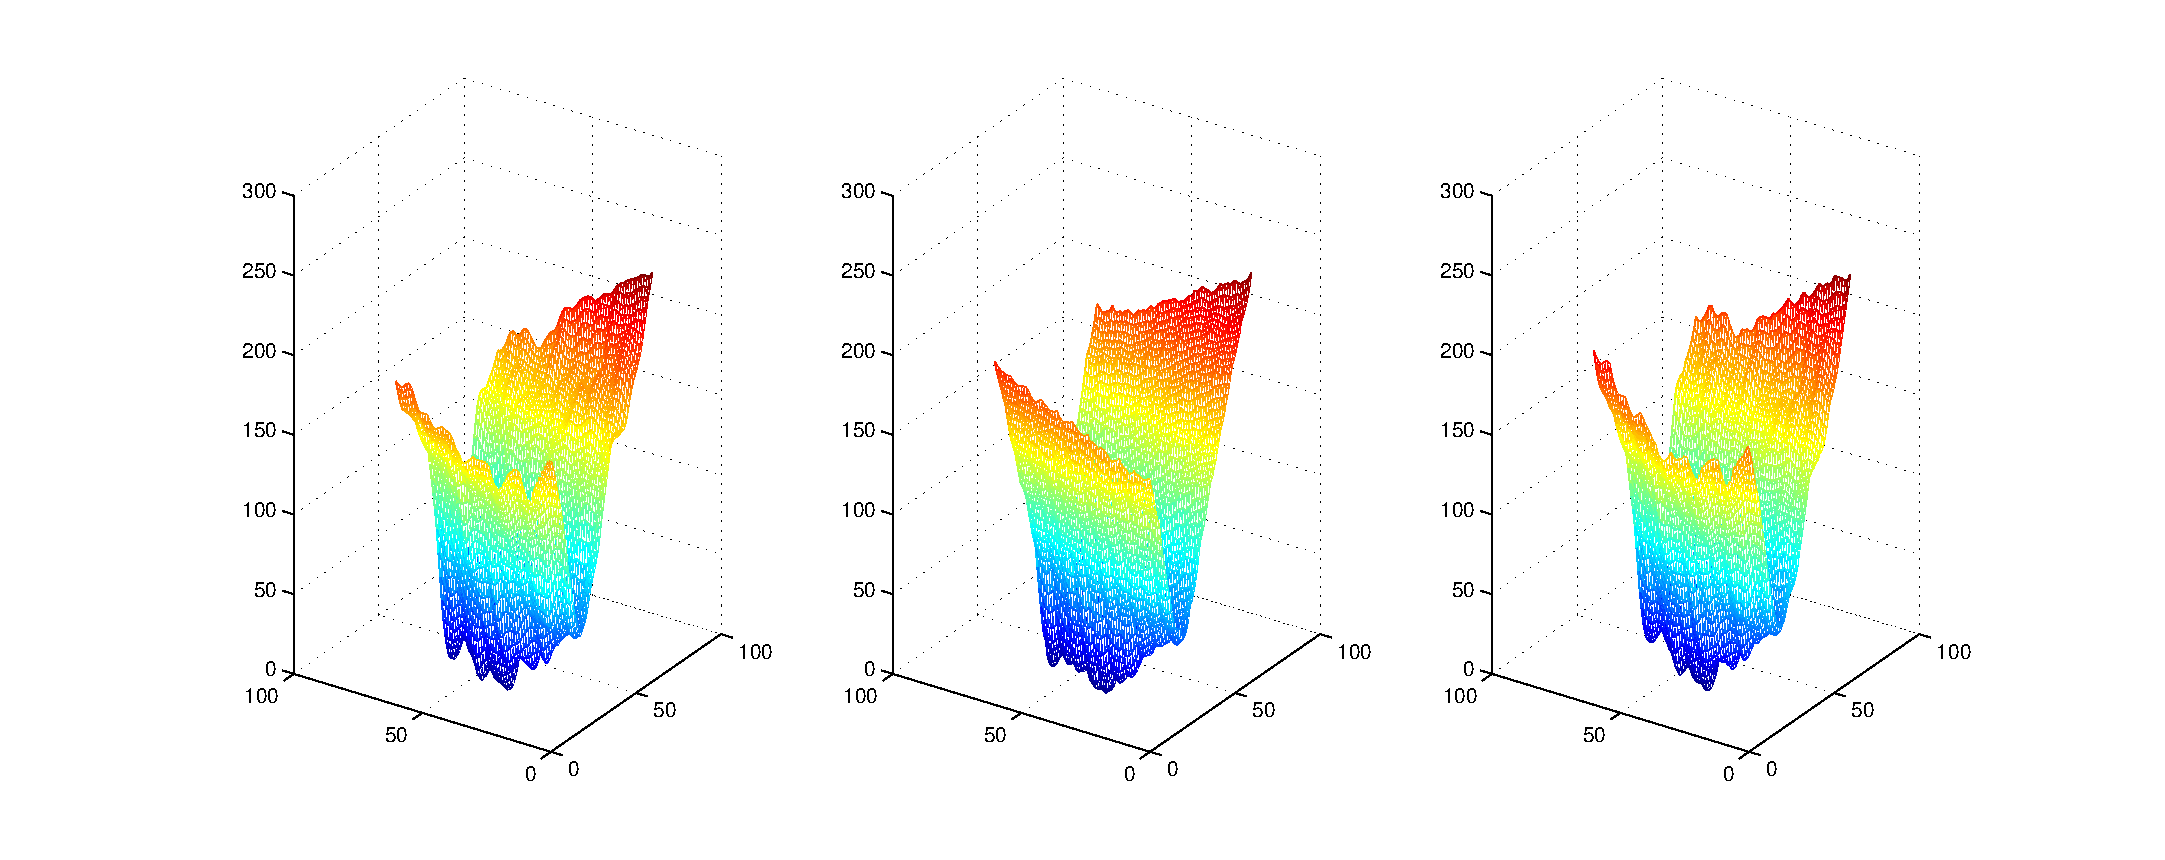
\includegraphics[width=0.95\textwidth]{pictures/Recal3DmetricsCMSReal}
\end{center}
\caption{Critères de différence pour une simulation de déplacement}{Valeur du critère de différence pour un déplacement réel entre deux images acquises à des instants différents.\\
De gauche à droite :\\
critère de \href{http://www.itk.org/Doxygen/html/classitk_1_1NormalizedCorrelationImageToImageMetric.html}{corrélation normalisé};\\
critère d'information mutuelle de \href{http://www.itk.org/Doxygen/html/classitk_1_1MattesMutualInformationImageToImageMetric.html}{Mattes};\\
critère des \href{http://www.itk.org/Doxygen/html/classitk_1_1MeanSquaresImageToImageMetric.html}{moindres carrés}. }
\label{fig:RecalMetricReal}
\end{figure}


La figure~\ref{fig:RecalMetricReal} montre que finalement, sur un essai réel, les trois critères présentent plusieurs minima locaux.
Nous utilisons pour l'instant le critère des moindres carrés pour sa simplicité théorique, mais nous envisageons d'utiliser d'autres critères si les expériences le mettent à défaut.


\subsubsection{Stabilisation de l'acquisition}

La stabilisation de l'acquisition est basée sur les mouvements précédents du spécimen :
nous corrigeons simplement la dernière translation. Le microscope a donc un échantillon de retard.

Afin de pouvoir intégrer la stabilisation au microscope, il a fallut programmer une extension du programme Megacapure.
Megacapture est un programme spécialement développé pour capturer et stocker
des vidéos tri-dimensionnelles de spécimen vivant.
Il a donc fallut intégrer la nouvelle fonctionnalité à Megacapture. Le programme de recalage a été codé en {\C++},
or Megacapture est une macro Visual Basic. il a donc fallu créer une interface.
J'ai travaillé avec Paul Cowgill pour créer une interface générique afin de connecter
Megacapture avec des programmes extérieurs. Cela permettant de respecter FC1 du diagramme pieuvre
(figure\ref{fig:PIEUVRERecal}).

\subsubsection{Avancement}

Nous sommes encore dans la phase d'intégration et de test sur ce projet.
Le programme de recalage a été crée, et connecté à Megacapture.
Il faut maintenant faire des expériences. Nous comptons tout d'abord tester le projet
sur des objets que nous bougerons manuellement, pour vérifier la réponse du Microscope.
Nous voulons ensuite tester notre programme sur un poisson zèbre en développement, au cours d'une session d'imagerie.

Il existe de nombreuses pistes pour étoffer les fonctionnalités de ce projet, en voici quelques unes :
\begin{itemize}
  \item Nous envisageons dans le futur d'utiliser un filtre de Kalman afin d'estimer
  le déplacement qui aura lieu à la prochaine acquisition, en connaissant les déplacements passés.
  \item Plutôt que d'utiliser un recalage rigide, il pourrait être judicieux d'utiliser un recalage "souple",
  qui donne un champ de déformation (déplacement de chaque point).
  Ainsi, le chercheur pourra sélectionner une zone d'intérêt sur un spécimen,
  et le programme, à partir du champ de déplacement dans cette région, pourra calculer
  le déplacement moyen de l'organe visé.
  \item Le temps d'exécution peut être raccourci en modifiant le programme pour qu'il soit multi-tâches.
  nous pouvons aussi améliorer la qualité du recalage en utilisant un débruitage et une réduction de la résolution
  des images à recaler, par ondelettes
  Cela nous permettrait d'obtenir une meilleure image grossière sur laquelle baser l'algorithme.
  \item Nous pouvons enfin utiliser un recalage "pyramidal" qui permet d'estimer tout premièrement un déplacement
  grossier (sur des images faible résolution), pour ensuite donner un recalage plus précis (sur des images haute résolution).
\end{itemize}


\section{Conclusion de la partie ingénierie du PFE}

Durant ce PFE, j'au travaillé sur des projets très variés.
Ces projets étaient motivés par des objectifs scientifiques et nécessitaient chacun un haut niveau de technicité.

J'ai eu l'occasion d'apprendre énormément,
notamment dans le domaine des sciences informatiques,
et du traitement de l'image.

J'ai aussi découvert le milieu de la recherche, dont l'organisation est
totalement différente de celle du milieu industriel.
La hiérarchie, et les intérêts de chaque scientifique sont moins apparents que dans une entreprise et ce PFE a été riche en enseignements sur ce plan.
Je suis parvenu à très bien m'intégrer dans l'équipe du Megason Lab en général,
et à établir de bonnes relations de travail avec les divers scientifiques
impliqués dans le projets sur lesquels j'ai travaillé, en particulier.

Cela m'a permis d'acquérir une base solide pour mener des recherches dans ce domaine.
Après une importante phase d'apprentissage, je maitrise maintenant des librairies de renom
(ITK, VTK,Qt), les systèmes unix, et la gestion de versions.

J'ai pu aussi établir des contacts dans la communauté
des traiteurs d'image par le biais de collaborations
(Matt MacCormick), ou de conférences internationales
(participation à la NAMIC summer project week, au MIT).
